\documentclass[titlepage]{book}

% PACKAGES

\usepackage[fontsize=13pt]{fontsize}
\usepackage{afterpage}
\usepackage{amsmath, amssymb}
\usepackage{slashed}
\usepackage[utf8]{inputenc}
\usepackage{chngcntr}
\usepackage{blindtext}
\usepackage[labelsep=space]{caption}
\usepackage{enumitem}
\usepackage{fancyhdr}
\usepackage[T1]{fontenc}
\usepackage[bottom=6.5em]{geometry}
\usepackage{graphicx}
\usepackage{gensymb}
\usepackage[hyperfootnotes=false,linktoc=page,pdfpagelayout=TwoPageRight]{hyperref}
\usepackage{lettrine}
% \usepackage{cfr-lm}
\usepackage{makecell}
\usepackage{mathtools}
\usepackage{multicol}
\usepackage[defaultlines=4,all]{nowidow}
\usepackage{titlesec}
\usepackage[titles]{tocloft}
\usepackage{wrapfig}
\usepackage{lipsum}
\usepackage{xcolor}
\usepackage{tikz-feynman}
\tikzfeynmanset{compat=1.1.0}
\usepackage{simpler-wick}
% IMPORTS

% MATH SHORTHANDS
% Partial Differential of #1 w.r.t. #2
\newcommand{\dpartial}[2]{\frac{\partial #1}{\partial #2}}

% \ceil{x} instead of \lceil x \rceil
% Same for \floor{x}
\DeclarePairedDelimiter\ceil{\lceil}{\rceil}
\DeclarePairedDelimiter\floor{\lfloor}{\rfloor}
\newcommand{\abs}[1]{\left| #1 \right|}

% Auto-resize () and []
\newcommand*\autoop{\left(}
\newcommand*\autocp{\right)}
\newcommand*\autoob{\left[}
\newcommand*\autocb{\right]}
\AtBeginDocument {%
   % \mathcode`( 32768
   % \mathcode`) 32768
   % \mathcode`[ 32768
   % \mathcode`] 32768
   \begingroup
       \lccode`\~`(
       \lowercase{%
   \endgroup
       \let~\autoop
   }\begingroup
       \lccode`\~`)
       \lowercase{%
   \endgroup
       \let~\autocp
   }\begingroup
       \lccode`\~`[
       \lowercase{%
   \endgroup
       \let~\autoob
   }\begingroup
       \lccode`\~`]
       \lowercase{%
   \endgroup
       \let~\autocb
}}
\delimiterfactor 1001
\makeatletter
\AtBeginDocument {%
          \def\resetMathstrut@{%
           \setbox\z@\hbox{\the\textfont\symoperators\char40}%
           \ht\Mathstrutbox@\ht\z@ \dp\Mathstrutbox@\dp\z@}%
}%
\makeatother

\newcommand{\vecbr}[1]{\langle #1 \rangle}

% Unit vectors

\newcommand{\ui}{\hat{\imath}}
\newcommand{\uj}{\hat{\jmath}}
\newcommand{\uk}{\hat{k}}
\newcommand{\V}{\vec{V}}

% Common expressions

\newcommand{\half}[1]{\frac{#1}{2}}
\newcommand{\recip}[1]{\frac{1}{#1}}
\newcommand{\invsqrt}[1]{\recip{\sqrt{#1}}}
\newcommand{\halfpi}{\half{\pi}}

% Integral evaluation bar
\newcommand{\windbar}[2]{\Big|_{#1}^{#2}}
\newcommand{\rightinfwindbar}[0]{\Big|_{0}^\infty}
\newcommand{\leftinfwindbar}[0]{\Big|_{-\infty}^0}

% Column type "L" for tabular environment, contents of column are in display mode by default
\newcolumntype{L}{>{$}l<{$}}

% Circled single character (used for state machine notation)

\newcommand{\state}[1]{\large\protect\textcircled{\textbf{\small#1}}}

% FORMATTING
% Remove section numbers
\makeatletter
\renewcommand{\@seccntformat}[1]{}
\makeatother
% Indent text within section
% \leftskip=2em
% Center section headings
\titleformat{\section}[block]{\Large\bfseries\filcenter}{}{1em}{}
% `enumerate` environment uses (\alph) format
\setlist[enumerate]{label=(\alph*)}

\newcommand{\shrule}{\\ \centerline{\rule{13cm}{0.4pt}}}

% QUANTUM

\usepackage{mathtools}
\DeclarePairedDelimiter\bra{\langle}{\rvert}
\DeclarePairedDelimiter\ket{\lvert}{\rangle}
\DeclarePairedDelimiterX\braket[2]{\langle}{\rangle}{#1 \delimsize\vert #2}
\DeclarePairedDelimiterX\brakaket[3]{\langle}{\rangle}{#1 \delimsize\vert #2 \delimsize\vert #3}
\newcommand{\tbra}[1]{$\bra{#1}$}
\newcommand{\tket}[1]{$\ket{#1}$}
\newcommand{\tbraket}[2]{$\braket{1}{2}$}
\newcommand{\infint}[0]{\int_{-\infty}^{\infty}}
\newcommand{\rightinfint}[0]{\int_0^\infty}
\newcommand{\leftinfint}[0]{\int_{-\infty}^0}
\newcommand{\wavefuncint}[1]{\infint|#1|^2}
\newcommand{\ham}[0]{\hat{H}}

\newcommand{\TODO}{\mathcal{TODO}}
\newcommand{\ud}{\mathrm{d}}
\newcommand{\mev}{\mathrm{MeV}}
\newcommand{\gev}{\mathrm{GeV}}
\renewcommand{\bf}[1]{\mathbf{#1}}
\newcommand{\condeq}[1]{\stackrel{=}{\mathclap{\substack{#1}}}}  % https://pbelmans.ncag.info/blog/2010/12/06/the-power-of-mathclap-and-substack/
\newcommand*\DAlambert{\mathop{}\!\mathbin\Box}


% PAGE HEADERS

\let\Sectionmark\sectionmark
\def\sectionmark#1{\def\Sectionname{#1}\Sectionmark{#1}}

\let\Subsectionmark\subsectionmark
\def\subsectionmark#1{\def\Subsectionname{#1}\Subsectionmark{#1}}

\pagestyle{fancy}
\fancyhf{}
\fancyhead[LE]{\thepage}
\fancyhead[RE]{\Sectionname}
\fancyhead[LO]{\MakeUppercase{\Subsectionname}}
\fancyhead[RO]{\thepage}
\renewcommand{\headrulewidth}{0pt}

% GRAPHICS

\graphicspath{ {./images/} }

% SECTION FORMAT

\counterwithout{subsection}{section}

\renewcommand{\thesection}{PART \Roman{section}}
\renewcommand{\thesubsection}{\Roman{subsection}}
\renewcommand{\thesubsubsection}{\Roman{subsubsection}}

\newcommand{\subsectionbreak}{\newpage}

\titleformat{\section}[display]{\Large\bfseries\filcenter}{\thesection}{.5em}{}
\titleformat{\subsection}[display]{\large\bfseries\filcenter}{\thesubsection}{0em}{\uppercase}

\counterwithin*{footnote}{page}

% FIGURES

\renewcommand{\thefigure}{\roman{figure}}

\renewcommand{\figurename}{\textsc{Fig.}}

\newcommand{\fig}[3]{
    \begin{figure}[h]
        \centering
        \includegraphics[width=\linewidth]{#1}
        \textbf{\caption{#2}}
        \label{fig:#3}
    \end{figure}
}

% EQUATIONS

\newcommand{\eq}[1]{
    \begin{equation*}
    \begin{split}
        #1
    \end{split}
    \end{equation*}
}

\newcommand{\eqnum}[1]{
    \begin{equation}
    \begin{split}
        #1
    \end{split}
    \end{equation}
}

% OLDSTYLENUMS

% \DeclareMathSymbol{0}{\mathalpha}{letters}{`0}
% \DeclareMathSymbol{1}{\mathalpha}{letters}{`1}
% \DeclareMathSymbol{2}{\mathalpha}{letters}{`2}
% \DeclareMathSymbol{3}{\mathalpha}{letters}{`3}
% \DeclareMathSymbol{4}{\mathalpha}{letters}{`4}
% \DeclareMathSymbol{5}{\mathalpha}{letters}{`5}
% \DeclareMathSymbol{6}{\mathalpha}{letters}{`6}
% \DeclareMathSymbol{7}{\mathalpha}{letters}{`7}
% \DeclareMathSymbol{8}{\mathalpha}{letters}{`8}
% \DeclareMathSymbol{9}{\mathalpha}{letters}{`9}

% REFERENCES

\hypersetup{
    colorlinks=false,
    linkbordercolor={0 0 0},
    pdfborderstyle={/S/U/W 0.0}
}

\newcommand{\secref}[1]{\hyperref[sec:#1]{Section #1}}

\newcommand{\figref}[1]{\hyperref[fig:#1]{Fig. #1}}

% LARGE FIRST LETTER OF SECTION

\newcommand{\firstword}[2]{
    \lettrine[lines=3,nindent=0em,findent=0.5em,realheight]{#1}{#2}
}

% TABLE OF CONTENTS FORMAT

\renewcommand{\contentsname}{CONTENTS}
\renewcommand{\cfttoctitlefont}{\hfil\bfseries\fontsize{15pt}{0pt}\selectfont}
\renewcommand{\cftaftertoctitleskip}{0.5\baselineskip}
\renewcommand{\cftsecfont}{\bfseries}

\addtolength{\cftsecnumwidth}{40pt}
\addtolength{\cftsubsecnumwidth}{10pt}
\setlength{\cftbeforetoctitleskip}{-3em}

\setcounter{tocdepth}{4}
\setcounter{secnumdepth}{4}

% TITLE SETUP

\title{\textbf{\huge{A cross section calculation handbook for students}}}

\author{
    Dacheng Xu
}

\date{}

% MISC

\newcommand{\aether}[0]{\ae ther}

\newcommand{\letlist}[1]{
    \begin{enumerate}[label=(\emph{\alph*})]
        #1
    \end{enumerate}
}

% DOCUMENT

\begin{document}

% TITLE

\maketitle

% PREFACE

\begin{center}
    \textbf{\Large{PREFACE}}
\end{center}

\firstword{T}{his} is a preface! \lipsum[1]

\vspace{\baselineskip}

\textit{Some Left Text, (Maybe a Date)} \hfill PREFACE AUTHOR

% TABLE OF CONTENTS

\pagenumbering{gobble}
\pagestyle{empty}
\newgeometry{bottom=6em}
\renewcommand{\baselinestretch}{0.94}\normalsize
\tableofcontents
\renewcommand{\baselinestretch}{1.0}\normalsize
\restoregeometry
\pagestyle{fancy}

\clearpage

% CONTENTS

\pagenumbering{arabic}

\section{Derivation}
\subsection{WIMP's interaction} \label{sec:wimp}

\subsubsection{Spin-independent WIMP-nucleon scattering}

% Using Helm's form factor\cite{helm_inelastic_1956}.

\clearpage

\subsection{Dark photon's interaction} \label{sec:dark_photon}

\clearpage

\subsection{Neutrino's interaction} \label{sec:neutrino}

Vertices and propagators in Glashow–Weinberg–Salam Theory:

Vertices:

\eqnum{
    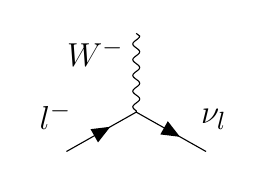
\begin{tikzpicture}
        \begin{feynman}
            \vertex(p) at (0, 0);
            \vertex(i) at (-0.886, -0.5);
            \vertex(f) at (0.886, -0.5);
            \vertex(o) at (0, 1);
            \diagram*{
                (i) --[fermion, edge label=$l^-$, near start] (p),
                (p) --[fermion, edge label=$\nu_l$, near end] (f),
                (p) --[boson, edge label=$W^-$, near end] (o),
            };
        \end{feynman}
    \end{tikzpicture},\quad
    \frac{-ig_W}{2\sqrt{2}}\gamma^\mu(1-\gamma^5)
}

\eqnum{
    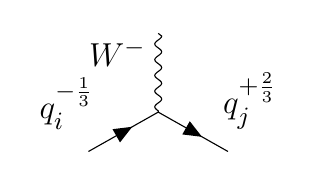
\begin{tikzpicture}
        \begin{feynman}
            \vertex(p) at (0, 0);
            \vertex(i) at (-0.886, -0.5);
            \vertex(f) at (0.886, -0.5);
            \vertex(o) at (0, 1);
            \diagram*{
                (i) --[fermion, edge label=$q_i^{-\recip{3}}$, near start] (p),
                (p) --[fermion, edge label=$q_j^{+\frac{2}{3}}$, near end] (f),
                (p) --[boson, edge label=$W^-$, near end] (o),
            };
        \end{feynman}
    \end{tikzpicture},\quad
    \frac{-ig_W}{2\sqrt{2}}\gamma^\mu(1-\gamma^5)V_{ij}
}

\eqnum{
    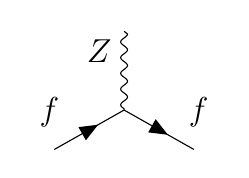
\begin{tikzpicture}
        \begin{feynman}
            \vertex(p) at (0, 0);
            \vertex(i) at (-0.886, -0.5);
            \vertex(f) at (0.886, -0.5);
            \vertex(o) at (0, 1);
            \diagram*{
                (i) --[fermion, edge label=$f$, near start] (p),
                (p) --[fermion, edge label=$f$, near end] (f),
                (p) --[boson, edge label=$Z$, near end] (o),
            };
        \end{feynman}
    \end{tikzpicture},\quad
    \frac{-ig_Z}{2}\gamma^\mu(c_V^f-c_A^f\gamma^5) = \frac{-ig_Z}{2}\gamma^\mu(I_3-2Q\sin^2{\theta_W}-I_3\gamma^5)
}

\begin{table}[htbp]
    \centering
    % \caption{}
    \begin{tabular}{|c c c|}
        \hline
        $f$ & $c_V$ & $c_A$ \\
        \hline
        $\nu_e,\nu_\mu,\nu_\tau$ & $\recip{2}$ & $\recip{2}$ \\
        \hline
        $e^-,\mu^-,\tau^-$ & $-\recip{2}+2\sin^2{\theta_W}$ & $-\recip{2}$ \\
        \hline
        $u,c,t$ & $\recip{2}-\frac{4}{3}\sin^2{\theta_W}$ & $\recip{2}$ \\
        \hline
        $d,s,b$ & $-\recip{2}+\frac{2}{3}\sin^2{\theta_W}$ & $-\recip{2}$ \\
        \hline
    \end{tabular}
\end{table}

Propagators:

\eqnum{
    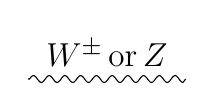
\begin{tikzpicture}
        \begin{feynman}
            \vertex(i) at (-1, 0);
            \vertex(f) at (1, 0);
            \diagram*{
                (i) --[boson, edge label=$W^{\pm}\,\mathrm{or}\,Z$] (f),
            };
        \end{feynman}
    \end{tikzpicture},\quad
    \frac{-i}{q^2-m^2}(g_{\mu\nu}-\frac{q_\mu q_\nu}{m^2})
}

when momentum of bosons is sufficiently low, the propagator is $\frac{ig_{\mu\nu}}{m^2}$.

\subsubsection{Neutrino-electron elastic scattering}

Neutrino-electron elastic scattering, commonly known as ES,
is the important neutral current events in several neutrino detection experiments,
such as Super-Kamiokande\cite{collaboration_solar_2001} and SNO\cite{sno_collaboration_direct_2002}.

The cross section is still related to the flavor of neutrinos.
$(\nu_e,e^-)$ has a 6.5 higher cross section than $(\nu_\mu,e^-)$ and $(\nu_\tau,e^-)$.

ES provides one of the key result of neutrino flux in the solar neutrino problem.

\eqnum{
    \nu_e + e^- \rightarrow \nu_e + e^-
}

\eqnum{
    & 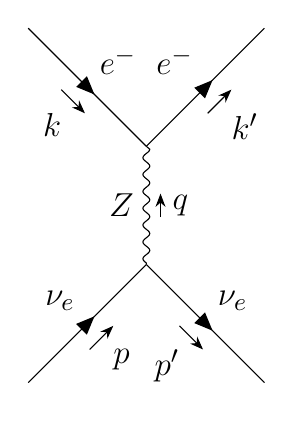
\begin{tikzpicture}[
        arrowlabel/.style={
            /tikzfeynman/momentum/.cd,
            arrow shorten=#1,
            arrow distance=0.6,
          },
          arrowlabel/.default=0.4
        ]
        \begin{feynman}
            \vertex(p1) at (0, 0);
            \vertex(p2) at (0, 1.5);
            \vertex(i1) at (-1.5, -1.5);
            \vertex(f1) at (1.5, -1.5);
            \vertex(i2) at (-1.5, 3);
            \vertex(f2) at (1.5, 3);
            \diagram*{
                (i1) --[fermion, edge label=$\nu_e$, momentum'={[arrowlabel]$p$}] (p1),
                (p1) --[fermion, edge label=$\nu_e$, momentum'={[arrowlabel]$p^\prime$}] (f1),
                (p1) --[boson, edge label=$Z$, momentum'={[arrowlabel]$q$}] (p2),
                (i2) --[fermion, edge label=$e^-$, momentum'={[arrowlabel]$k$}] (p2),
                (p2) --[fermion, edge label=$e^-$, momentum'={[arrowlabel]$k^\prime$}] (f2),
            };
        \end{feynman}
    \end{tikzpicture} \\
    =& u^s(p)\frac{-ig_Z}{2}\gamma^\mu(\recip{2}-\recip{2}\gamma^5)\bar{u}^{s^\prime}(p^\prime)
    \frac{ig_{\mu\nu}}{m_Z^2}
    \bar{u}^r(k)\frac{-ig_Z}{2}\gamma^\nu(c_V-c_A\gamma^5)u^{r^\prime}(k^\prime)
}

The amplitude:

\eqnum{
    \label{eq:amp_ES}
    i\mathcal{M} =& -i\frac{g_Z^2}{4m_Z^2}u^s(p)\gamma^\mu(\recip{2}-\recip{2}\gamma^5)\bar{u}^{s^\prime}(p^\prime)
    \bar{u}^r(k)\gamma_\nu(c_V-c_A\gamma^5)u^{r^\prime}(k^\prime)
}

Importantly, electrons have two states of spins. But neutrinos, as massless particles, only have one state of spin,
they are always left-handed and polarized, so the spin sum of all states is:

\eqnum{
    \langle\abs{M}^2\rangle = \sum_{s}\sum_{s^\prime}\half{1}\sum_{r}\sum_{r^\prime}\abs{M(s,s^\prime\rightarrow r,r^\prime)}^2.
}

Similar to 5.2 in Peskin's book,

\eqnum{
    \label{eq:M_ES_1}
    &\langle\abs{M}^2\rangle \\
    =& \recip{2^7}(\frac{g_Z}{m_Z})^4
    \left(u^s(p)\gamma^\mu(1-\gamma^5)\bar{u}^{s^\prime}(p^\prime)u^{s^\prime}(p^\prime)(1-\gamma^5)\bar{u}^s(p)\gamma^\nu\right) \\
    &\cdot\left(\bar{u}^r(k)\gamma_\mu(c_V-c_A\gamma^5)u^{r^\prime}(k^\prime)\bar{u}^{r^\prime}(k^\prime)(c_V-c_A\gamma^5)u^r(k)\gamma_\nu\right) \\
    =& \recip{2^7}(\frac{g_Z}{m_Z})^4
    \mathrm{tr}\left[(\slashed{p}+m_\nu)\gamma^\mu(1-\gamma^5)(\slashed{p}^\prime+m_\nu)\gamma^\nu(1-\gamma^5)\right] \\
    &\cdot \mathrm{tr}\left[(\slashed{k}+m_e)\gamma_\mu(c_V-c_A\gamma^5)(\slashed{k}^\prime+m_e)\gamma_\nu(c_V-c_A\gamma^5)\right]
}

Proof a lemma, a useful general case for traces in week interaction:

\eqnum{
    &\mathrm{tr}\left[(\slashed{p}+m)\gamma^\mu(c_V-c_A\gamma^5)(\slashed{p}^\prime+m^\prime)\gamma^\nu(c_V-c_A\gamma^5)\right] \\
    =& \mathrm{tr}\left[\slashed{p}\gamma^\mu c_V\slashed{p}^\prime\gamma^\nu c_V\right]
    - \mathrm{tr}\left[\slashed{p}\gamma^\mu c_V\slashed{p}^\prime\gamma^\nu c_A\gamma^5\right] \\
    &+ \mathrm{tr}\left[\slashed{p}\gamma^\mu c_V m^\prime \gamma^\nu c_V\right]
    - \mathrm{tr}\left[\slashed{p}\gamma^\mu c_V m^\prime \gamma^\nu c_A\gamma^5\right] \\
    &- \mathrm{tr}\left[\slashed{p}\gamma^\mu c_A\gamma^5\slashed{p}^\prime\gamma^\nu c_V\right]
    + \mathrm{tr}\left[\slashed{p}\gamma^\mu c_A\gamma^5\slashed{p}^\prime\gamma^\nu c_A\gamma^5\right] \\
    &- \mathrm{tr}\left[\slashed{p}\gamma^\mu c_A\gamma^5 m^\prime \gamma^\nu c_V\right]
    + \mathrm{tr}\left[\slashed{p}\gamma^\mu c_A\gamma^5 m^\prime \gamma^\nu c_A\gamma^5\right] \\
    &+ \mathrm{tr}\left[m\gamma^\mu c_V\slashed{p}^\prime\gamma^\nu c_V\right]
    - \mathrm{tr}\left[m\gamma^\mu c_V\slashed{p}^\prime\gamma^\nu c_A\gamma^5\right] \\
    &+ \mathrm{tr}\left[m\gamma^\mu c_V m^\prime \gamma^\nu c_V\right]
    - \mathrm{tr}\left[m\gamma^\mu c_V m^\prime \gamma^\nu c_A\gamma^5\right] \\
    &- \mathrm{tr}\left[m\gamma^\mu c_A\gamma^5\slashed{p}^\prime\gamma^\nu c_V\right]
    + \mathrm{tr}\left[m\gamma^\mu c_A\gamma^5\slashed{p}^\prime\gamma^\nu c_A\gamma^5\right] \\
    &- \mathrm{tr}\left[m\gamma^\mu c_A\gamma^5 m^\prime \gamma^\nu c_V\right]
    + \mathrm{tr}\left[m\gamma^\mu c_A\gamma^5 m^\prime \gamma^\nu c_A\gamma^5\right] \\
    =& \mathrm{tr}\left[\slashed{p}\gamma^\mu c_V\slashed{p}^\prime\gamma^\nu c_V\right]
    - \mathrm{tr}\left[\slashed{p}\gamma^\mu c_V\slashed{p}^\prime\gamma^\nu c_A\gamma^5\right] \\
    &+ 0
    - 0 \\
    &- \mathrm{tr}\left[\slashed{p}\gamma^\mu c_A\gamma^5\slashed{p}^\prime\gamma^\nu c_V\right]
    + \mathrm{tr}\left[\slashed{p}\gamma^\mu c_A\gamma^5\slashed{p}^\prime\gamma^\nu c_A\gamma^5\right] \\
    &- 0
    + 0 \\
    &+ 0
    - 0 \\
    &+ \mathrm{tr}\left[m\gamma^\mu c_V m^\prime \gamma^\nu c_V\right]
    - 0 \\
    &- 0
    + 0 \\
    &- 0
    + \mathrm{tr}\left[m\gamma^\mu c_A\gamma^5 m^\prime \gamma^\nu c_A\gamma^5\right]
}

We can wait a sec here to calculate another quantity we will use later, from 5.5 in Peskin's book:

\eqnum{
    &\mathrm{tr}\left[\slashed{p}\gamma^\mu \slashed{p}^\prime\gamma^\nu \right] \\
    =& \mathrm{tr}\left[\gamma^\rho \gamma^\mu \gamma^\sigma \gamma^\nu \right]p_\rho p_\sigma^\prime \\
    =& 4(g^{\rho\mu}g^{\sigma\nu}-g^{\rho\sigma}g^{\mu\nu}+g^{\rho\nu}g^{\mu\sigma})p_\rho p_\sigma^\prime \\
    =& 4(p^\mu p^{\prime\nu} - p\cdot p^\prime g^{\mu\nu} + p^\nu p^{\prime\mu}).
}

We should noticed that $\mathrm{tr}\left[\slashed{p}\gamma^\mu c_V\slashed{p}^\prime\gamma^\nu c_V\right]$
and $\mathrm{tr}\left[\slashed{p}\gamma^\mu c_A\gamma^5\slashed{p}^\prime\gamma^\nu c_A\gamma^5\right]$ looks similar,
both with even $\gamma^\mu$ and even $\gamma^5$, actually they are the same except $c_V \rightarrow c_A$.
Because $\{\gamma^\nu,\gamma^5\}=0$.

The nasty term:

\eqnum{
    &\mathrm{tr}\left[\slashed{p}\gamma^\mu c_V\slashed{p}^\prime\gamma^\nu c_A\gamma^5\right] \\
    =& -4i c_V c_A \epsilon^{\rho\mu\sigma\nu}p_\rho p^\prime_\sigma \\
    =& \mathrm{tr}\left[\slashed{p}\gamma^\mu c_A\gamma^5\slashed{p}^\prime\gamma^\nu c_V\right]
}

Easier terms:

\eqnum{
    \mathrm{tr}\left[m\gamma^\mu c_V m^\prime \gamma^\nu c_V\right] = 4m m^\prime c_V^2 g^{\mu\nu}
}

\eqnum{
    &\mathrm{tr}\left[m\gamma^\mu c_A\gamma^5 m^\prime \gamma^\nu c_A\gamma^5\right] \\
    =& -4m m^\prime c_A^2 \mathrm{tr}\left[\gamma^\mu \gamma^\nu \gamma^5 \gamma^5\right] \\
    =& -4m m^\prime c_A^2 \mathrm{tr}\left[\gamma^\mu \gamma^\nu \right] \\
    =& -4m m^\prime c_A^2 g^{\mu\nu}
}

So:

\eqnum{
    &\mathrm{tr}\left[(\slashed{p}+m)\gamma^\mu(c_V-c_A\gamma^5)(\slashed{p}^\prime+m^\prime)\gamma^\mu(c_V-c_A\gamma^5)\right] \\
    =& 4c_V^2(p^\mu p^{\prime\nu} - p\cdot p^\prime g^{\mu\nu} + p^\nu p^{\prime\mu})
    + 4c_A^2(p^\mu p^{\prime\nu} - p\cdot p^\prime g^{\mu\nu} + p^\nu p^{\prime\mu}) \\
    & +8i c_V c_A \epsilon^{\rho\mu\sigma\nu} \\
    & +4m m^\prime (c_V^2-c_A^2) g^{\mu\nu} \\
    =& 4(c_V^2+c_A^2)(p^\mu p^{\prime\nu} + p^\nu p^{\prime\mu} - p\cdot p^\prime g^{\mu\nu})
    + 4m m^\prime (c_V^2-c_A^2) g^{\mu\nu} \\
    & +8i c_V c_A \epsilon^{\mu\nu\rho\sigma}p_\rho p^\prime_\sigma
}

Plugin the lemma back to \eqref{eq:M_ES_1}:

\eqnum{
    &\langle\abs{M}^2\rangle \\
    =& \recip{2^7}(\frac{g_Z}{m_Z})^4\left[
        8(p^\mu p^{\prime\nu} + p^\nu p^{\prime\mu} - (p\cdot p^\prime)g^{\mu\nu})
        + 8i \epsilon^{\mu\nu\rho\sigma}p_\rho p^\prime_\sigma
    \right] \\
    & \cdot \left[
        4(c_V^2+c_A^2)(k_\mu k^\prime_\nu + k_\nu k^\prime_\mu - (k\cdot k^\prime) g_{\mu\nu})
        + 4 m_e^2 (c_V^2-c_A^2) g_{\mu\nu}
        + 8i c_V c_A \epsilon_{\mu\nu\alpha\beta} k^\alpha k^{\prime\beta}
    \right] \\
    =& \recip{4}(\frac{g_Z}{m_Z})^4\left[
        (p^\mu p^{\prime\nu} + p^\nu p^{\prime\mu} - (p\cdot p^\prime)g^{\mu\nu})
        + i \epsilon^{\mu\nu\rho\sigma}p_\rho p^\prime_\sigma
    \right] \\
    & \cdot \left[
        (c_V^2+c_A^2)(k_\mu k^\prime_\nu + k_\nu k^\prime_\mu - (k\cdot k^\prime) g_{\mu\nu})
        +  m_e^2 (c_V^2-c_A^2) g_{\mu\nu}
        + 2i c_V c_A \epsilon_{\mu\nu\alpha\beta} k^\alpha k^{\prime\beta}
    \right]
}

We have the following tricks:

\eqnum{
    g_{\mu\nu}\epsilon^{\mu\nu\rho\sigma} &= 0 \\
    \epsilon^{\mu\nu\rho\sigma}p_\rho p^\prime_\sigma(k_\mu k^\prime_\nu + k_\nu k^\prime_\mu) &= 0 \\
    \epsilon_{\mu\nu\alpha\beta} k^\alpha k^{\prime\beta}(p^\mu p^{\prime\nu} + p^\nu p^{\prime\mu}) &= 0 \\
    \epsilon^{\mu\nu\rho\sigma}\epsilon_{\mu\nu\alpha\beta} &=
    -2(\delta^\rho_{\phantom{x}\alpha}\delta^\sigma_{\phantom{x}\beta}
    - \delta^\rho_{\phantom{x}\beta}\delta^\sigma_{\phantom{x}\alpha})
}

So:

\eqnum{
    \label{eq:M_ES_2}
    &\langle\abs{M}^2\rangle \\
    =& \recip{4}(\frac{g_Z}{m_Z})^4\left[
        (p^\mu p^{\prime\nu} + p^\nu p^{\prime\mu} - (p\cdot p^\prime)g^{\mu\nu})
        + i \epsilon^{\mu\nu\rho\sigma}p_\rho p^\prime_\sigma
    \right] \\
    & \cdot \left[
        (c_V^2+c_A^2)(k_\mu k^\prime_\nu + k_\nu k^\prime_\mu - (k\cdot k^\prime) g_{\mu\nu})
        + m_e^2 (c_V^2-c_A^2) g_{\mu\nu}
        + 2i c_V c_A \epsilon_{\mu\nu\alpha\beta} k^\alpha k^{\prime\beta}
    \right] \\
    =& \recip{4}(\frac{g_Z}{m_Z})^4\left[
        2(c_V^2+c_A^2)(
            (p\cdot k)(p^\prime\cdot k^\prime) + (p\cdot k^\prime)(p^\prime\cdot k) - (p\cdot p^\prime)(k\cdot k^\prime) \right. \\
            &+ (p\cdot k^\prime)(p^\prime\cdot k) + (p\cdot k)(p^\prime\cdot k^\prime) - (p\cdot p^\prime)(k\cdot k^\prime) \\
            &- (p\cdot p^\prime)(k\cdot k^\prime) - (p\cdot p^\prime)(k\cdot k^\prime) + 4(p\cdot p^\prime)(k\cdot k^\prime)) \\
        & m_e^2 (c_V^2-c_A^2)(2(p\cdot p^\prime)-4(p\cdot p^\prime)) \\
        &- \left. 2 c_V c_A\epsilon^{\mu\nu\rho\sigma}\epsilon_{\mu\nu\alpha\beta} p_\rho p^\prime_\sigma k^\alpha k^{\prime\beta}
    \right] \\
    =& \recip{2}(\frac{g_Z}{m_Z})^4\left[
        (c_V^2+c_A^2)((p\cdot k)(p^\prime\cdot k^\prime) + (p\cdot k^\prime)(p^\prime\cdot k)) \right. \\
        &- m_e^2 (c_V^2-c_A^2)(p\cdot p^\prime) \\
        &+ \left. 2 c_V c_A (\delta^\rho_{\phantom{x}\alpha}\delta^\sigma_{\phantom{x}\beta}
        - \delta^\rho_{\phantom{x}\beta}\delta^\sigma_{\phantom{x}\alpha})p_\rho p^\prime_\sigma k^\alpha k^{\prime\beta}
    \right] \\
    =& \recip{2}(\frac{g_Z}{m_Z})^4\left[
        (c_V+c_A)^2(p\cdot k)(p^\prime\cdot k^\prime) + (c_V-c_A)^2(p\cdot k^\prime)(p^\prime\cdot k) \right. \\
        &- \left. m_e^2 (c_V^2-c_A^2)(p\cdot p^\prime)
    \right]
}

In ES experiments, usually the energy of neutrino is large, e.g. the solar neutrinos are $\sim\mathrm{MeV}$ neutrinos.
So in center-of-mass frame(CM), we can ignore the mass of electron, i.e. $m_e=0$, and set(similar to 5.62 in Peskin's book):

\eqnum{
    p &= (x, x\hat{z}) \\
    p^\prime &= (x, \bf{x}) \\
    k &= (E, -x\hat{z}) \\
    k^\prime &= (E, -\bf{x}).
}

So that:

\eqnum{
    x &= E \\
    \bf{x}\cdot\hat{z} &= x\cos{\theta} \\
    (p\cdot k) &= (p^\prime\cdot k^\prime) = x(E+x) \\
    (p\cdot k^\prime) &= (p^\prime\cdot k) = x(E+x\cos{\theta})
}

Note that if here we set the mass of electron to be zero,
then we would not be able to get a differential cross section as function of the recoil energy, because there is no energy exchange.

\eqnum{
    &\langle\abs{M}^2\rangle \\
    =& \recip{2}(\frac{g_Z}{m_Z})^4\left[
    (c_V+c_A)^2(p\cdot k)(p^\prime\cdot k^\prime) + (c_V-c_A)^2(p\cdot k^\prime)(p^\prime\cdot k) \right. \\
    &- \left. m_e^2 (c_V^2-c_A^2)(p\cdot p^\prime)
    \right] \\
    =& 2(\frac{g_Z E}{m_Z})^4\left[(c_V+c_A)^2 + (c_V-c_A)^2(\half{1+\cos{\theta}})^2\right] \\
    =& 2(\frac{g_Z E}{m_Z})^4\left[(c_V+c_A)^2 + (c_V-c_A)^2\cos^4{\half{\theta}}\right]
}

From 4.84 in Peskin's book:

\eqnum{
    &\left(\frac{\ud\sigma}{\ud\Omega}\right)_{\mathrm{CM}} \\
    =& \frac{\abs{\mathcal{M}}^2}{64\pi^2(E+x)^2} \\
    =& \recip{128\pi^2}(\frac{g_Z}{m_Z})^4 E^2 \left[(c_V+c_A)^2 + (c_V-c_A)^2\cos^4{\half{\theta}}\right] \\
    \propto & E^2
}

and the total cross section is:

\eqnum{
    &\sigma_{\mathrm{total}} \\
    =& \recip{24\pi}(\frac{g_Z}{m_Z})^4 E^2 \left[c_V^2 + c_A^2 + c_V c_A\right]
}

\begin{figure}[htbp]
    \centering
    \includesvg[width=\linewidth]{images/es_comparison.svg}
    \caption{Comparison between ES in derivation and literate\cite{akimov_coherent_2018}}
    \label{fig:es_comparison}
\end{figure}

Fig.~\ref{fig:es_comparison} shows the comparison between this result and result from literature.
The difference between them might comes from the too-simplified tree level derivation.

\subsubsection{Coherent elastic neutrino-nucleus scattering}

Coherent elastic neutrino-nucleus scattering, commonly known as CE$\nu$NS,
is an important irreducible background in the drak matter direct detection experiments,
such as XENON1T\cite{aprile_search_2021} and PandaX-4T\cite{ma_search_2023}.
The process has already been observed by COHERENT\cite{akimov_observation_2017} at the
Spallation Neutron Source (SNS) at Oak Ridge National Laboratory.

To derive the cross section of such interaction,
we skip the stringent tree-level derivation but borrow the result from last section.

\eqnum{
    & 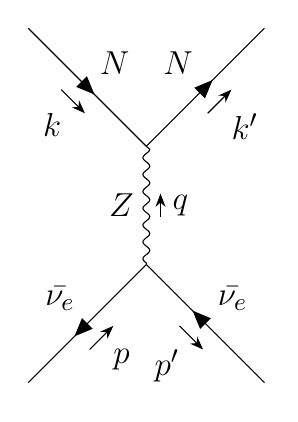
\begin{tikzpicture}[
        arrowlabel/.style={
            /tikzfeynman/momentum/.cd,
            arrow shorten=#1,
            arrow distance=0.6,
          },
          arrowlabel/.default=0.4
        ]
        \begin{feynman}
            \vertex(p1) at (0, 0);
            \vertex(p2) at (0, 1.5);
            \vertex(i1) at (-1.5, -1.5);
            \vertex(f1) at (1.5, -1.5);
            \vertex(i2) at (-1.5, 3);
            \vertex(f2) at (1.5, 3);
            \diagram*{
                (i1) --[anti fermion, edge label=$\bar{\nu_e}$, momentum'={[arrowlabel]$p$}] (p1),
                (p1) --[anti fermion, edge label=$\bar{\nu_e}$, momentum'={[arrowlabel]$p^\prime$}] (f1),
                (p1) --[boson, edge label=$Z$, momentum'={[arrowlabel]$q$}] (p2),
                (i2) --[fermion, edge label=$N$, momentum'={[arrowlabel]$k$}] (p2),
                (p2) --[fermion, edge label=$N$, momentum'={[arrowlabel]$k^\prime$}] (f2),
            };
        \end{feynman}
    \end{tikzpicture} \\
    =& \bar{v}^s(p)\frac{-ig_Z}{2}\gamma^\mu(\recip{2}-\recip{2}\gamma^5)v^{s^\prime}(p^\prime)
    \frac{ig_{\mu\nu}}{m_Z^2}
    \bar{u}^r(k)\frac{-ig_Z}{2}\gamma^\nu(c_V-c_A\gamma^5)u^{r^\prime}(k^\prime) \\
    =& \bar{v}^s(p)\frac{-ig_Z}{2}\gamma^\mu(\recip{2}-\recip{2}\gamma^5)v^{s^\prime}(p^\prime)
    \frac{ig_{\mu\nu}}{m_Z^2}
    \bar{u}^r(k)\frac{-ig_Z}{2}\gamma^\nu(I_3-2Q\sin^2{\theta_W}-I_3\gamma^5)u^{r^\prime}(k^\prime)
}

$I_3$ is the weak isospin, $Q$ is the charge. For neutron, the vertex is:

\eqnum{
    -i\frac{g_Z}{2}\gamma^\mu\left(-\recip{2}+\half{\gamma^5}\right),
}

for proton, the vertex is:

\eqnum{
    -i\frac{g_Z}{2}\gamma^\mu\left(\recip{2}-2\sin^2{\theta_W}-\half{\gamma^5}\right),
}

for neutrino, the vertex is:

\eqnum{
    -i\frac{g_Z}{2}\gamma^\mu\left(\recip{2}-\half{\gamma^5}\right).
}

Even if we use anti-electron neutrino here, the derivation is still similar to the derivation of ES.
The only deterrence is that we need to take into account all the protons and neutrons inside the nuclei.
Also we need to introduce a form factor because the nuclei is not a point particle.
Copy equation from \eqref{eq:M_ES_2}, this is for each nucleon:

\eqnum{
    &\langle\abs{M}^2\rangle \\
    =& \recip{2}(\frac{g_Z}{m_Z})^4\left[
        (c_V+c_A)^2(p\cdot k)(p^\prime\cdot k^\prime) + (c_V-c_A)^2(p\cdot k^\prime)(p^\prime\cdot k) \right. \\
        &- \left. m^2 (c_V^2-c_A^2)(p\cdot p^\prime)
    \right],
}

where m is the mass of nucleon.

In lab frame, similar to 5.88 in Peskin's book:

\eqnum{
    p &= (\omega, \omega\hat{z}) \\
    p^\prime &= (\omega^\prime, \omega^\prime\sin{\theta},0,\omega^\prime\cos{\theta}) \\
    k &= (m, \bf{0}) \\
    k^\prime &= (E^\prime, \bf{k^\prime})
}

\todo[inline]{Finish total and differential CEvNS cross section calculation and compare to literatures.}

\subsubsection{Inverse beta decay}

\clearpage

\subsection{Axion's interaction} \label{sec:axion}


\section{Miscellaneous}
\subsection{Derivation of equations in Peskin's book}

% TODO: add reference to the textbooks
There are many equations which are not detailedly derived in Peskin's book.

Here I first revisit the equation 2.30 and 2.31:

Given

\eqnum{
    \omega_{\bf{p}} =& \sqrt{\abs{\bf{p}}+m^2}
}

\eqnum{
    \phi(\bf{x}) =& \int\frac{\ud^3p}{(2\pi)^3}\recip{\sqrt{2\omega_{\bf{p}}}}(a_{\bf{p}}+a^\dagger_{-\bf{p}})e^{i\bf{p}\cdot\bf{x}}
}

\eqnum{
    \pi(\bf{x}) =& \int\frac{\ud^3p}{(2\pi)^3}(-i)\sqrt{\frac{\omega_{\bf{p}}}{2}}(a_{\bf{p}}-a^\dagger_{-\bf{p}})e^{i\bf{p}\cdot\bf{x}}
}

\eqnum{
    \left[a_{\bf{p}},a^\dagger_{\bf{p^\prime}}\right] =& (2\pi)^3\delta^{(3)}(\bf{p}-\bf{p^\prime})
}

\eqnum{
    \left[\phi(\bf{x}),\pi(\bf{x^\prime})\right]
    =& \int\frac{\ud^3p\ud^3p^\prime}{(2\pi)^6}
    \frac{-i}{2}\sqrt{\frac{\omega_{\bf{p^\prime}}}{\omega_{\bf{p}}}}
    \left(
        \left[a^\dagger_{-\bf{p}},a_{\bf{p^\prime}}\right]-\left[a_{\bf{p}},a^\dagger_{-\bf{p^\prime}}\right]
    \right)e^{i(\bf{p}\bf{x}+\bf{p^\prime}\bf{x^\prime})} \\
    =& \int\frac{\ud^3p\ud^3p^\prime}{(2\pi)^3}
    \frac{-i}{2}\sqrt{\frac{\omega_{\bf{p^\prime}}}{\omega_{\bf{p}}}}
    \left[
        -\delta^{(3)}(-\bf{p}-\bf{p^\prime})-\delta^{(3)}(\bf{p}+\bf{p^\prime})
    \right]e^{i(\bf{p}\bf{x}+\bf{p^\prime}\bf{x^\prime})} \\
    =& i\int\frac{\ud^3p\ud^3p^\prime}{(2\pi)^3}
    \sqrt{\frac{\omega_{\bf{p^\prime}}}{\omega_{\bf{p}}}}
    \delta^{(3)}(\bf{p}+\bf{p^\prime})
    e^{i(\bf{p}\bf{x}+\bf{p^\prime}\bf{x^\prime})} \\
    =& i\int\frac{\ud^3p}{(2\pi)^3}
    e^{i\bf{p}(\bf{x}-\bf{x^\prime})} \\
    =& i\delta^{(3)}(\bf{x}-\bf{x^\prime})
}

from equation 2.8,

\eqnum{
    H =& \int\ud^3x\mathcal{H} \\
    =& \int\ud^3x\left[\half{1}\pi^2+\half{1}(\nabla\phi)^2+\half{1}m^2\phi^2\right] \\
    =& \int\ud^3xe^{i(\bf{p}+\bf{p^\prime})\cdot\bf{x}}\int\frac{\ud^3p\ud^3p^\prime}{(2\pi)^6}
    \{
        -\frac{\sqrt{\omega_{\bf{p}}\omega_{\bf{p^\prime}}}}{4}
        (a_{\bf{p}}-a^\dagger_{-\bf{p}})(a_{\bf{p^\prime}}-a^\dagger_{-\bf{p^\prime}}) \\
        &+ \frac{-\bf{p}\cdot\bf{p^\prime}+m^2}{4\sqrt{\omega_{\bf{p}}\omega_{\bf{p^\prime}}}}
        (a_{\bf{p}}+a^\dagger_{-\bf{p}})(a_{\bf{p^\prime}}+a^\dagger_{-\bf{p^\prime}})
    \} \\
    =& \int\frac{\ud^3p\ud^3p^\prime}{(2\pi)^6}
    \{
        -\frac{\sqrt{\omega_{\bf{p}}\omega_{\bf{p^\prime}}}}{4}
        (a_{\bf{p}}-a^\dagger_{-\bf{p}})(a_{\bf{p^\prime}}-a^\dagger_{-\bf{p^\prime}}) \\
        &+ \frac{-\mathbf{p}\cdot\mathbf{p^\prime}+m^2}{4\sqrt{\omega_{\bf{p}}\omega_{\bf{p^\prime}}}}
        (a_{\bf{p}}+a^\dagger_{-\bf{p}})(a_{\bf{p^\prime}}+a^\dagger_{-\bf{p^\prime}})
    \}(2\pi)^3\delta^{(3)}(\bf{p}+\bf{p^\prime}) \\
    =& \int\frac{\ud^3p}{(2\pi)^3}
    \left[
        -\frac{\omega_{\bf{p}}}{4}
        (a_{\bf{p}}-a^\dagger_{-\bf{p}})(a_{-\bf{p}}-a^\dagger_{\bf{p}})
        + \frac{\abs{\bf{p}}+m^2}{4\omega_{\bf{p}}}
        (a_{\bf{p}}+a^\dagger_{-\bf{p}})(a_{-\bf{p}}+a^\dagger_{\bf{p}})
    \right] \\
    =& -\int\frac{\ud^3p}{(2\pi)^3}\recip{4\omega_{\bf{p}}}
    \{
        (\abs{\bf{p}}^2+m^2)\left[(a_{\bf{p}}-a^\dagger_{-\bf{p}})(a_{-\bf{p}}-a^\dagger_{\bf{p}})
        - (a_{\bf{p}}+a^\dagger_{-\bf{p}})(a_{-\bf{p}}+a^\dagger_{\bf{p}})\right]
    \} \\
    =& \int\frac{\ud^3p}{(2\pi)^3}\half{\omega_{\bf{p}}}
    \left(a_{\bf{p}}a_{\bf{p^\prime}}+a_{-\bf{p}}a_{-\bf{p^\prime}}\right) \\
    =& \int\frac{\ud^3p}{(2\pi)^3}\omega_{\bf{p}}
    \left(a_{\bf{p^\prime}}a_{\bf{p}}+\half{1}\left[a_{\bf{p}},a_{\bf{p^\prime}}\right]\right)
}

Revisit the equation 2.46:

Given

\eqnum{
    H^na_{\bf{p}} =& a_{\bf{p}}(H-E_{\bf{p}})^n
}

So

\eqnum{
    e^{iHt}a_{\bf{p}} =& a_{\bf{p}}e^{i(H-E_{\bf{p}})t}
}

Then

\eqnum{
    e^{iHt}a_{\bf{p}}e^{-iHt} =& a_{\bf{p}}e^{-iE_{\bf{p}}t}
}

Revisit the equation 2.54:

When $x^0>y^0$,

\eqnum{
    \infint\ud p^0\recip{p^2-m^2}e^{-ip\cdot(x-y)}
    =& \int\ud p^0\recip{{p^0}^2-\bf{p}^2-m^2}e^{-ip\cdot(x-y)} \\
    =& -\half{1}(2\pi i)
    \{
        \mathop{\mathrm{Res}}(\recip{{p^0}^2-\bf{p}^2-m^2},-E_{\bf{p}}) \\
        &+ \mathop{\mathrm{Res}}(\recip{{p^0}^2-\bf{p}^2-m^2},E_{\bf{p}})
    \}e^{-ip\cdot(x-y)}
}

following the contour in the book, which goes around the poles \textcolor{red}{clockwise}.

\eqnum{
    \brakaket{0}{\left[\phi(x),\phi(y)\right]}{0}
    =& \int\frac{\ud^3p}{(2\pi)^3}\recip{2E_{\bf{p}}}\left(e^{-ip\cdot(x-y)}-e^{ip\cdot(x-y)}\right) \\
    =& \int\frac{\ud^3p}{(2\pi)^3}
    \{
        \recip{2E_{\bf{p}}}e^{-ip\cdot(x-y)}\vert_{p^0=E_{\bf{p}}} \\
        &+ \recip{-2E_{\bf{p}}}e^{-ip\cdot(x-y)}\vert_{p^0=-E_{\bf{p}}}
    \} \\
    \condeq{x^0>y^0\ \ }& \int\frac{\ud^3p}{(2\pi)^3}\int\frac{\ud p^0}{2\pi i}\frac{-1}{p^2-m^2}e^{-ip\cdot(x-y)}
}

Revisit the equation 2.58:

Given

\eqnum{
    D_R(x-y) =& \int\frac{\ud^4p}{(2\pi)^4}e^{-ip\cdot(x-y)}\tilde{D}_R(p)
}

Set $(x-y)$ as $\Delta x$

\eqnum{
    \tilde{D}_R(p^\prime)
    =& \int\ud^4\Delta x\int\frac{\ud^3p}{(2\pi)^3}\recip{2E_{\bf{p}}}
    \left(
        e^{-ip\cdot\Delta x} - e^{ip\cdot\Delta x}
    \right)e^{ip^\prime} \\
    =& \int\ud\Delta x^{(0)}\int\ud^3p
    \left(
        \left[\delta^(3)(\bf{p^\prime}-\bf{p})e^{-i{p^\prime}^{(0)}}-\delta^(3)(\bf{p^\prime}+\bf{p})e^{i{p^\prime}^{(0)}}\right]
    \right) \\
    =& \int\ud\Delta x^{(0)}\recip{2E_{\bf{p^\prime}}}\left(e^{-iE_{\bf{p^\prime}}\Delta x^{(0)}}-e^{iE_{\bf{p^\prime}}\Delta x^{(0)}}\right) \\
    =& \recip{2E_{\bf{p^\prime}}}\left(\recip{-iE_{\bf{p^\prime}}}-\recip{iE_{\bf{p^\prime}}}\right) \\
    =& \frac{i}{E_{\bf{p^\prime}}^2}
}

Revisit the formula between 3.5 and 3.6, it is from 2.45. 

Revisit 3.17, David Tong's Claim 4.2.

Revisit 3.29, 3.34  % TODO

Revisit 3.50:

\eqnum{
    u(p)
    =& \begin{pmatrix}
        \sqrt{p\cdot\sigma}\xi \\
        \sqrt{p\cdot\bar{\sigma}}\xi
    \end{pmatrix} \\
    =& \begin{pmatrix}
        \sqrt{
            \bigl(\begin{smallmatrix}
                E+p^3 & \\
                & E-p^3
            \end{smallmatrix}\bigr)
        }\xi \\
        \sqrt{
            \bigl(\begin{smallmatrix}
                E-p^3 & \\
                & E+p^3
            \end{smallmatrix}\bigr)
        }\xi
    \end{pmatrix} \\
    =& \begin{pmatrix}
        \bigl(\begin{smallmatrix}
            \sqrt{E+p^3} & \\
            & \sqrt{E-p^3}
        \end{smallmatrix}\bigr)\xi \\
        \bigl(\begin{smallmatrix}
            \sqrt{E-p^3} & \\
            & \sqrt{E+p^3}
        \end{smallmatrix}\bigr)\xi
    \end{pmatrix} \\
    =& \begin{pmatrix}
        \left[
            \sqrt{E+p^3}\left(\half{1-\sigma^3}\right) + \sqrt{E-p^3}\left(\half{1+\sigma^3}\right)
        \right]\xi \\
        \left[
            \sqrt{E-p^3}\left(\half{1+\sigma^3}\right) + \sqrt{E+p^3}\left(\half{1-\sigma^3}\right)
        \right]\xi
    \end{pmatrix}
}

Revisit 3.65:

\eqnum{
    u^{r\dagger}(p)v^s(p)
    =& \begin{pmatrix}
        \xi^{r\dagger}\sqrt{p\cdot\sigma}, \xi^{r\dagger}\sqrt{p\cdot\bar{\sigma}}
    \end{pmatrix}
    \cdot
    \begin{pmatrix}
        \sqrt{p\cdot\sigma}\xi^{s} \\
        -\sqrt{p\cdot\bar{\sigma}}\xi^{s}
    \end{pmatrix} \\
    =& \begin{pmatrix}
        E+p^3 & \\
        & E-p^3
    \end{pmatrix}\delta^{rs}
     - \begin{pmatrix}
        E-p^3 & \\
        & E+p^3
    \end{pmatrix}\delta^{rs} \\
    \neq& 0
}

\eqnum{
    u^{r\dagger}(\bf{p})v^s(-\bf{p})
    =& \begin{pmatrix}
        E-p^3 & \\
        & E+p^3
    \end{pmatrix}\delta^{rs}
     - \begin{pmatrix}
        E+p^3 & \\
        & E-p^3
    \end{pmatrix}\delta^{rs} \\
    =& 0
}


% \section{PART TITLE}

\subsection{CHAPTER TITLE} \label{sec:I}

\firstword{M}{ore} big letter text. \lipsum[5] 

Lettered List: 

\letlist{
    \item \lipsum[1]
    \item \lipsum[2-2]
    \item \lipsum[3-3]
}

\subsection{NEXT CHAPTER TITLE}

\firstword{H}{ere} is an example of a chapter reference: \secref{I}. \lipsum[1]

\lipsum[2-2] \textbf{An example of a centered equation:} \[
    t' = \frac{t - \frac{v}{c^2}x}{\sqrt{1 - \frac{v^2}{c^2}}}
\]

\lipsum[3-3] \textbf{An example of an inline equation:} $x = -\frac{\pm \sqrt{b^2 - 4ac}}{2a}$ \lipsum[4-4]. \textbf{Now we have a footnote}\footnote{Hello! Example equations down here also: $\ham \psi = \hat{E}\psi$.}.

An example figure: \fig{fig1}{An Example Figure Caption}{i}

If I want to reference it, \figref{i}.

Unnumbered equations:\eq{
    x = y \\
    y = z \\
    x = z \\
}

Numbered group of equations:\eqnum{
    a = b \\
    b = c \\
    a = c \\
}


\end{document}
